\documentclass{TDP003mall}
\usepackage{float}


\newcommand{\version}{Version 1.1}
\author{Arturas Aleksandrauskas, \url{artal938@student.liu.se}\\
  Joakim Johansson, \url{joajo229@student.liu.se}}
\title{ANVÄNDARMANUAL}
\date{2016-09-05}
\rhead{Arturas Aleksandrauskas\\
Joakim Johansson}



\begin{document}
\projectpage


\section{Header, meny och footer}
/\textit{på alla sidor}

I headern ska det finnas en bild på personen som ägen hemsidan och även en titel och slogan som denne får hitta på. Titeln ska vara länkad till root-sidan på ``/''. 

Menyn ska vara en simpel menu som är horisontellt centrerad och det ska finnas någon enkel ``hover'' effekt. Det ska finnas länkar till List, Tekniker och Home. De ska såklart vara länkade till deras respective sidor.

I footern ska det står basic information om copyright och vem som gjort hemsidan och vilket år den vart skapad.


\section{Home}
\textit{/}

På första sidan ska det finnas en liten text ``Om mig'' och sedan ska det även finnas en lista på de senaste projekten som lagts upp på sidan, detta för att det ska upplevas lite mer dynamiskt och att det känns som att det händer något på hemsidan, att den är aktiv liksom. Varje projekt som visas på sidan ska ha en enkel beskrivning, namn, datum, vilka teknikern den använder, en bild och även en knapp som går till en sida där man ska kunna läsa mer om projektet.

Varje teknik ``text''  ska också ha en länk på sig som går till sidan för tekniker där den skrollar ner automatiskt till den tekniken så att man kan se fler projekt som använder samma teknik.

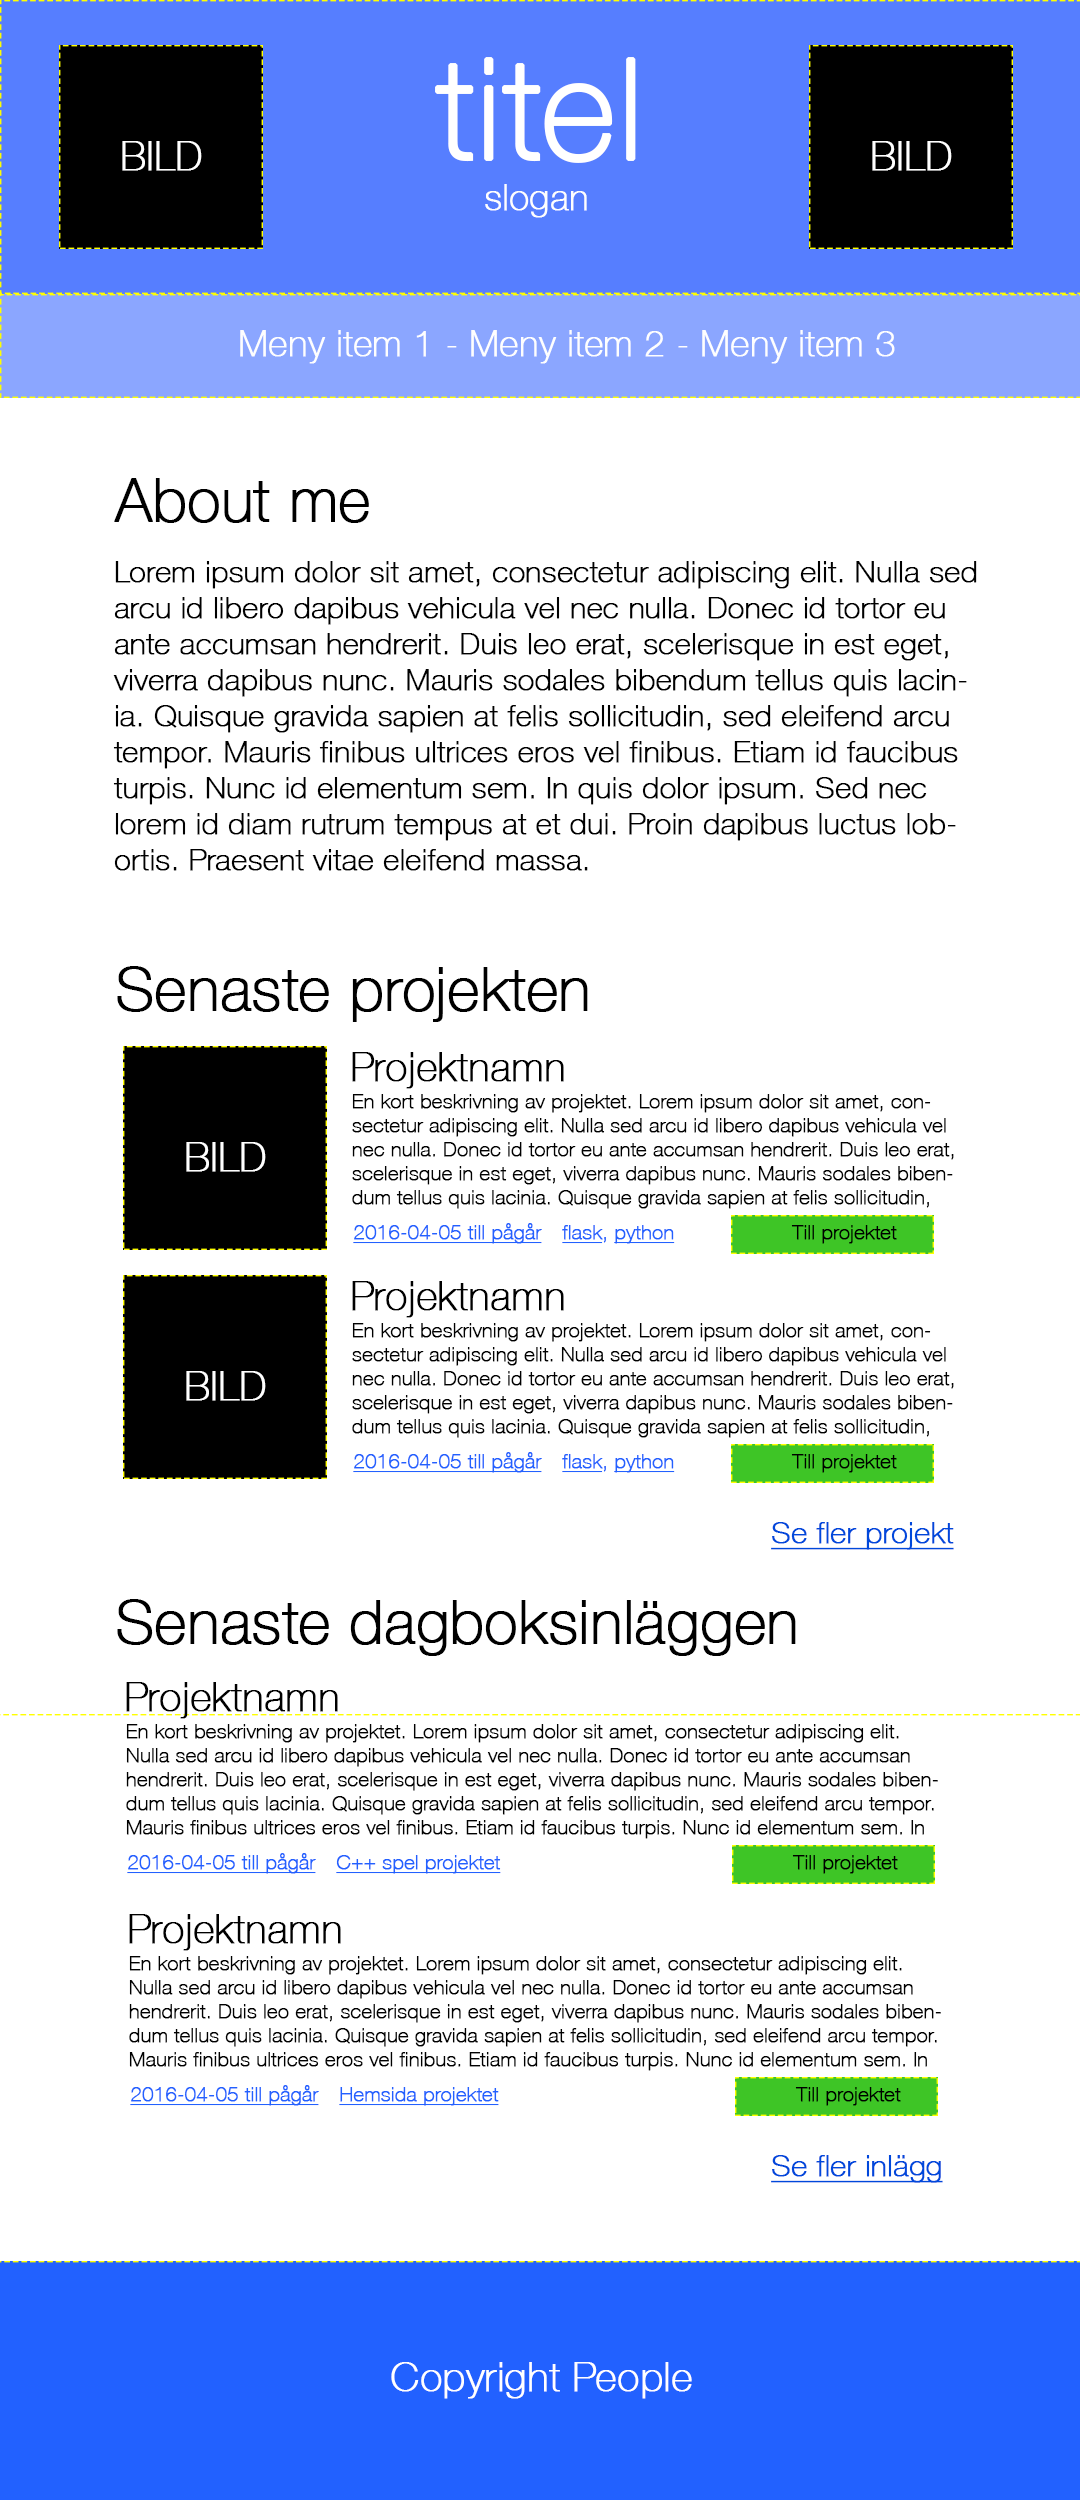
\includegraphics[height=14cm]{index.png}

\section{Lista på projekten}
\textit{/list}

List sidan ska vara en lång lista på alla projekt som finns på hemsidan. Man ska kunna klicka på varje projekt, antigen på bilden, titeln eller knappen för att komma till sidan för just det specifika projektet.

Man ska även kunna sorta lista på datum, vilken typ av teknik som ska vara med. Man ska även kunna skriva in ett sökord och då ska den bara ta med de projekt där söknyckeln finns med i.

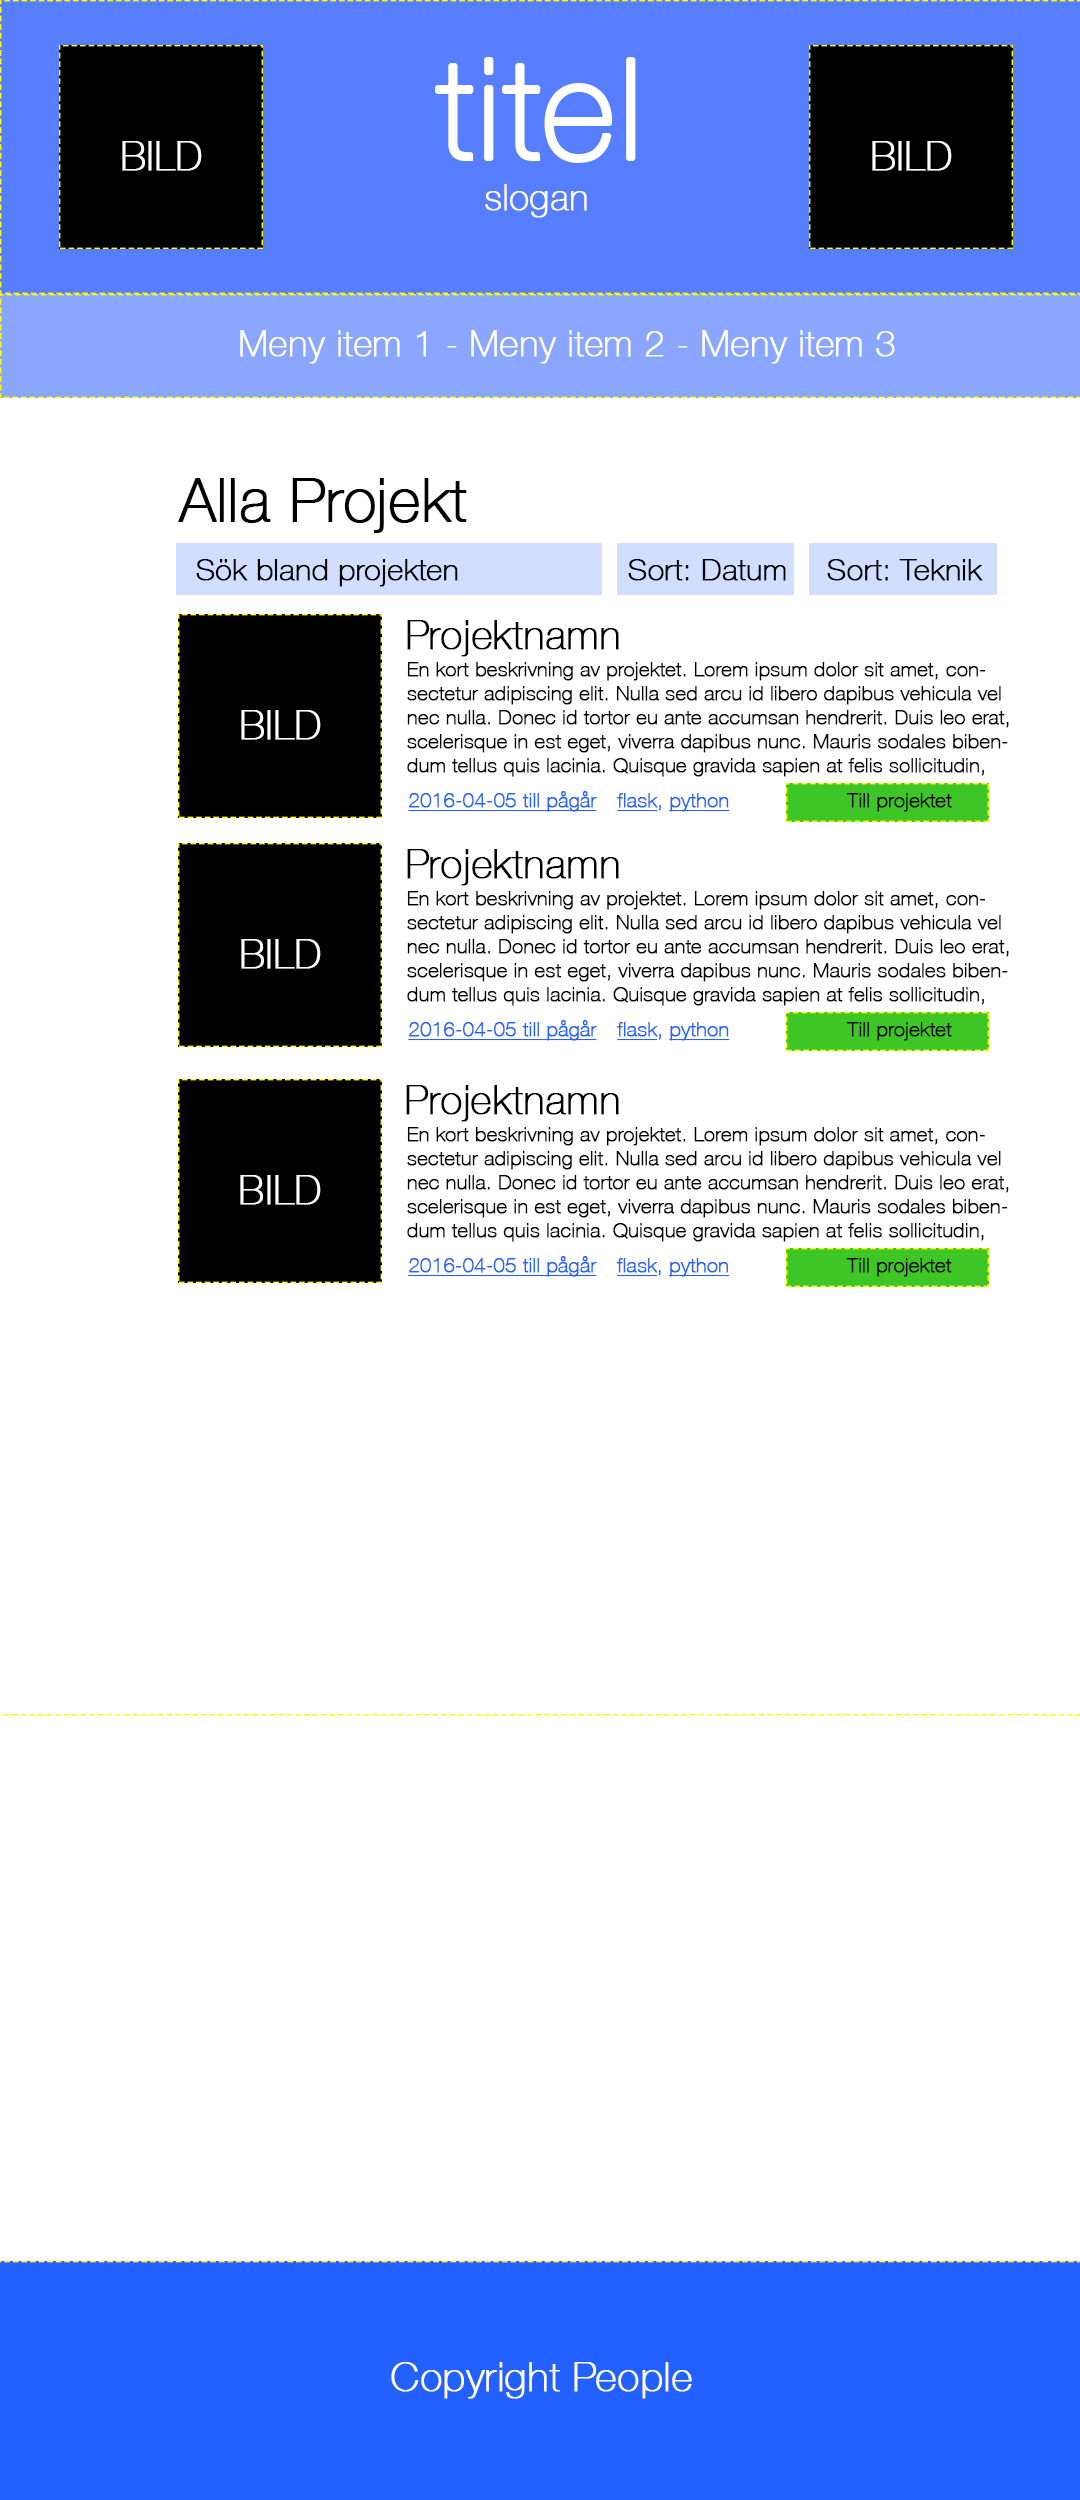
\includegraphics[height=14cm]{list.png}


\section{Lista på teknikerna och dess projekt}
\textit{/technoligys}

På denna sida så ska det finnas en lista på alla tekniker som finns med i projekten och sedan under varje teknik så ska det finnas en liten lista på alla de projekt som använder den tekniken. Man ska kunna klicka på varje projekt och då komma till dessas egna sidor. Denna sida ska även ha id:n i html:en vid varje teknik-titel, så att man ska kunna länka till en specifik teknik.

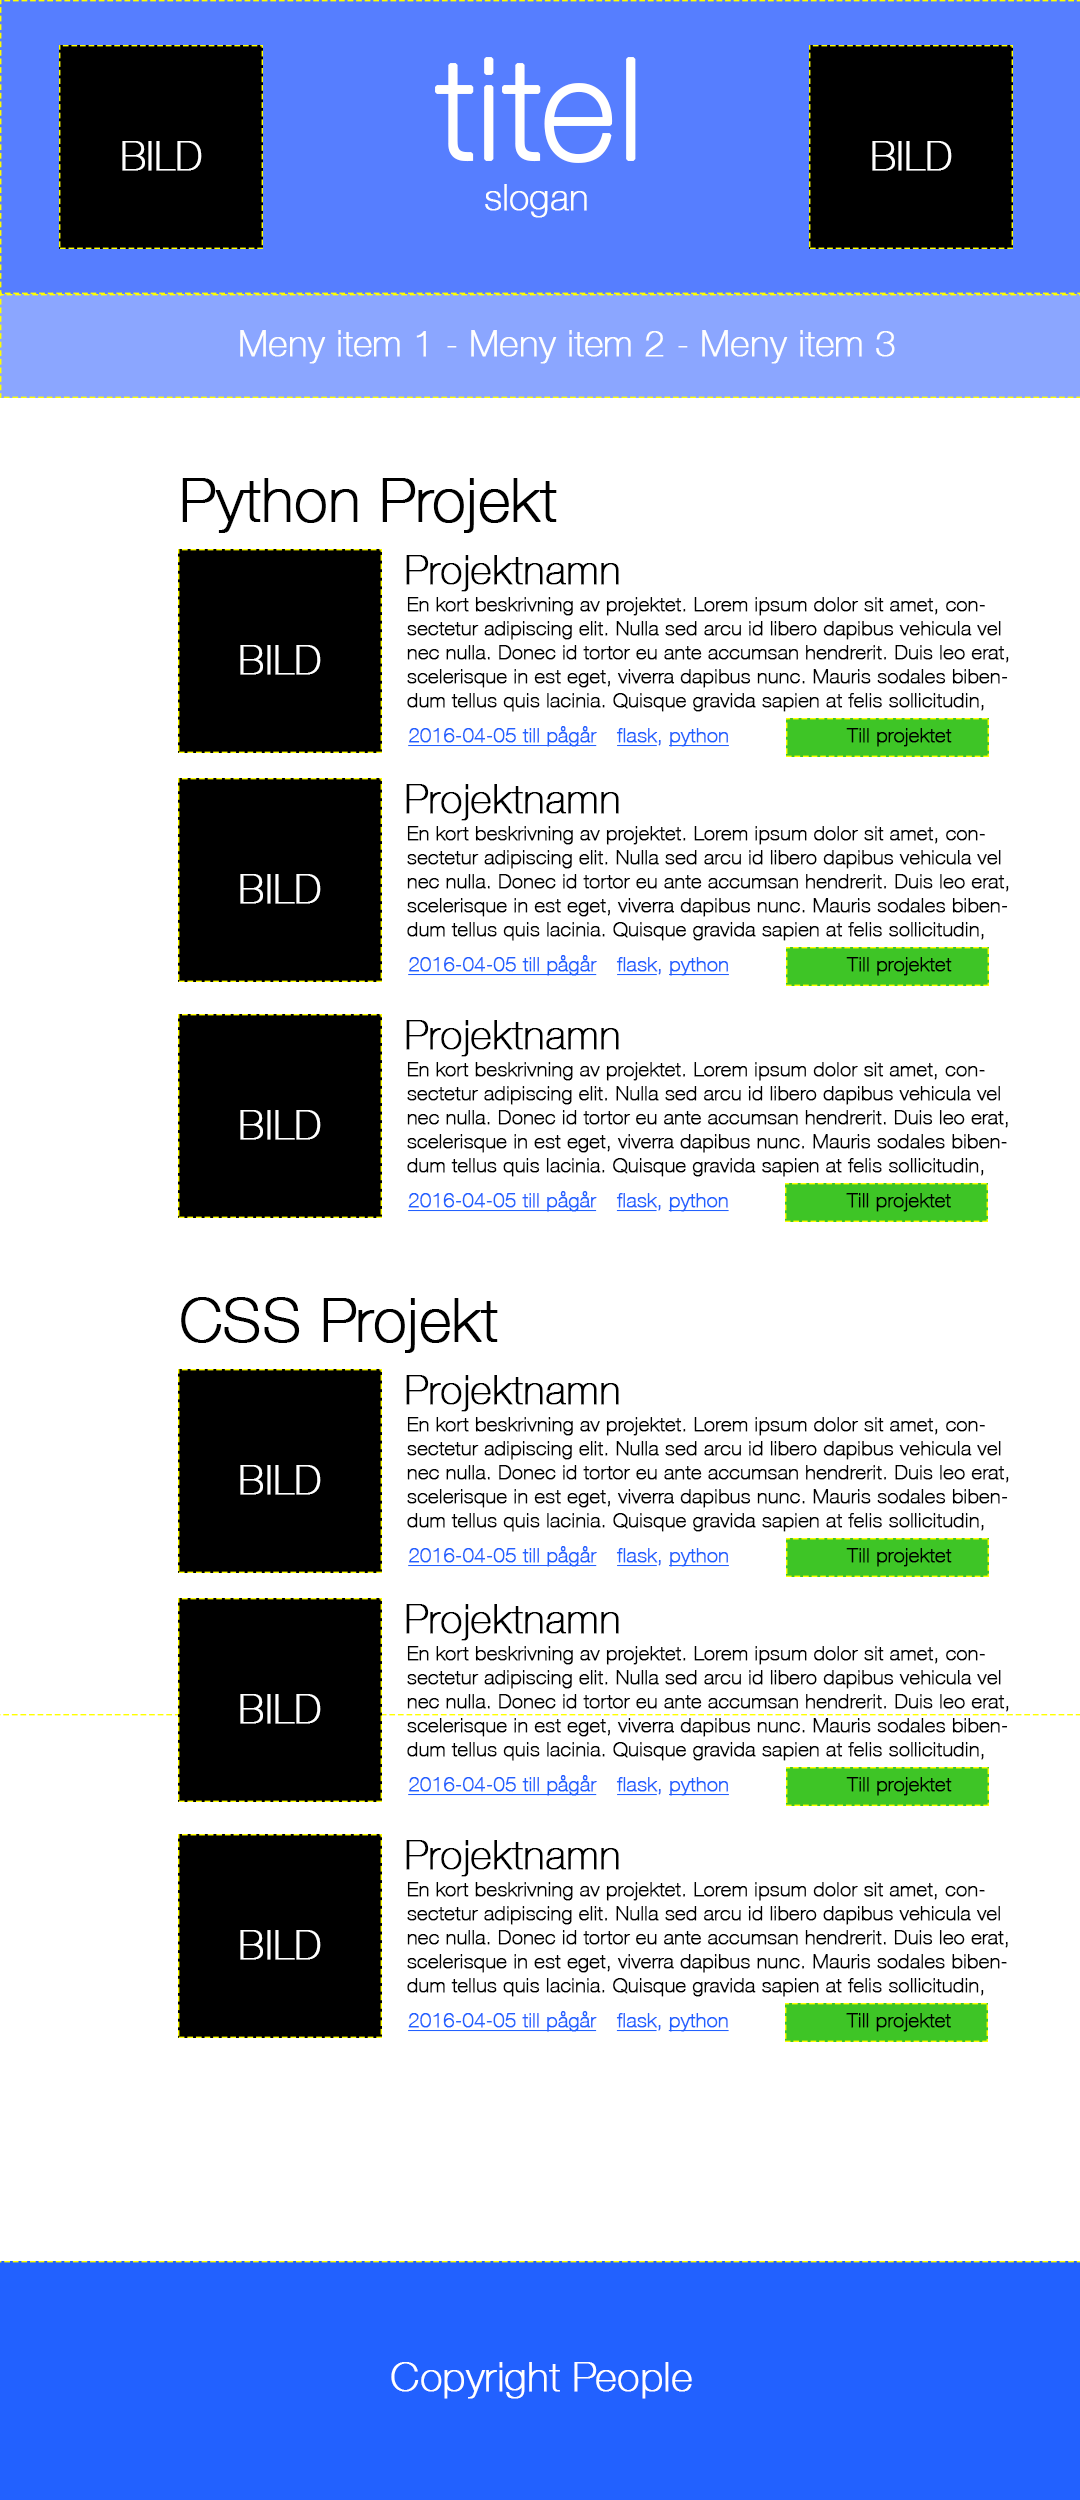
\includegraphics[height=14cm]{tekniker.png}


\section{Ett projekt}
\textit{/project/id}

På projekt/id sida så ska den visa det projekt som har det id som man skriv in i URL:en. Här ska all information om det aktuella projektet finnas.

Det ska finnas en bild, titel, den fulla beskrivningen, sourcefilerna med kod och även en sidebar med lite kortare information så som datum, personer som gjort projektet, kurskod, tekniker som använts(länkade till tekniksidan(hashtag)teknik) och licens som koden är under.

(Vi hade tänkte att ha en dagboksfunktion men vi skippar det till en början och gör bara den om vi får tid över.)

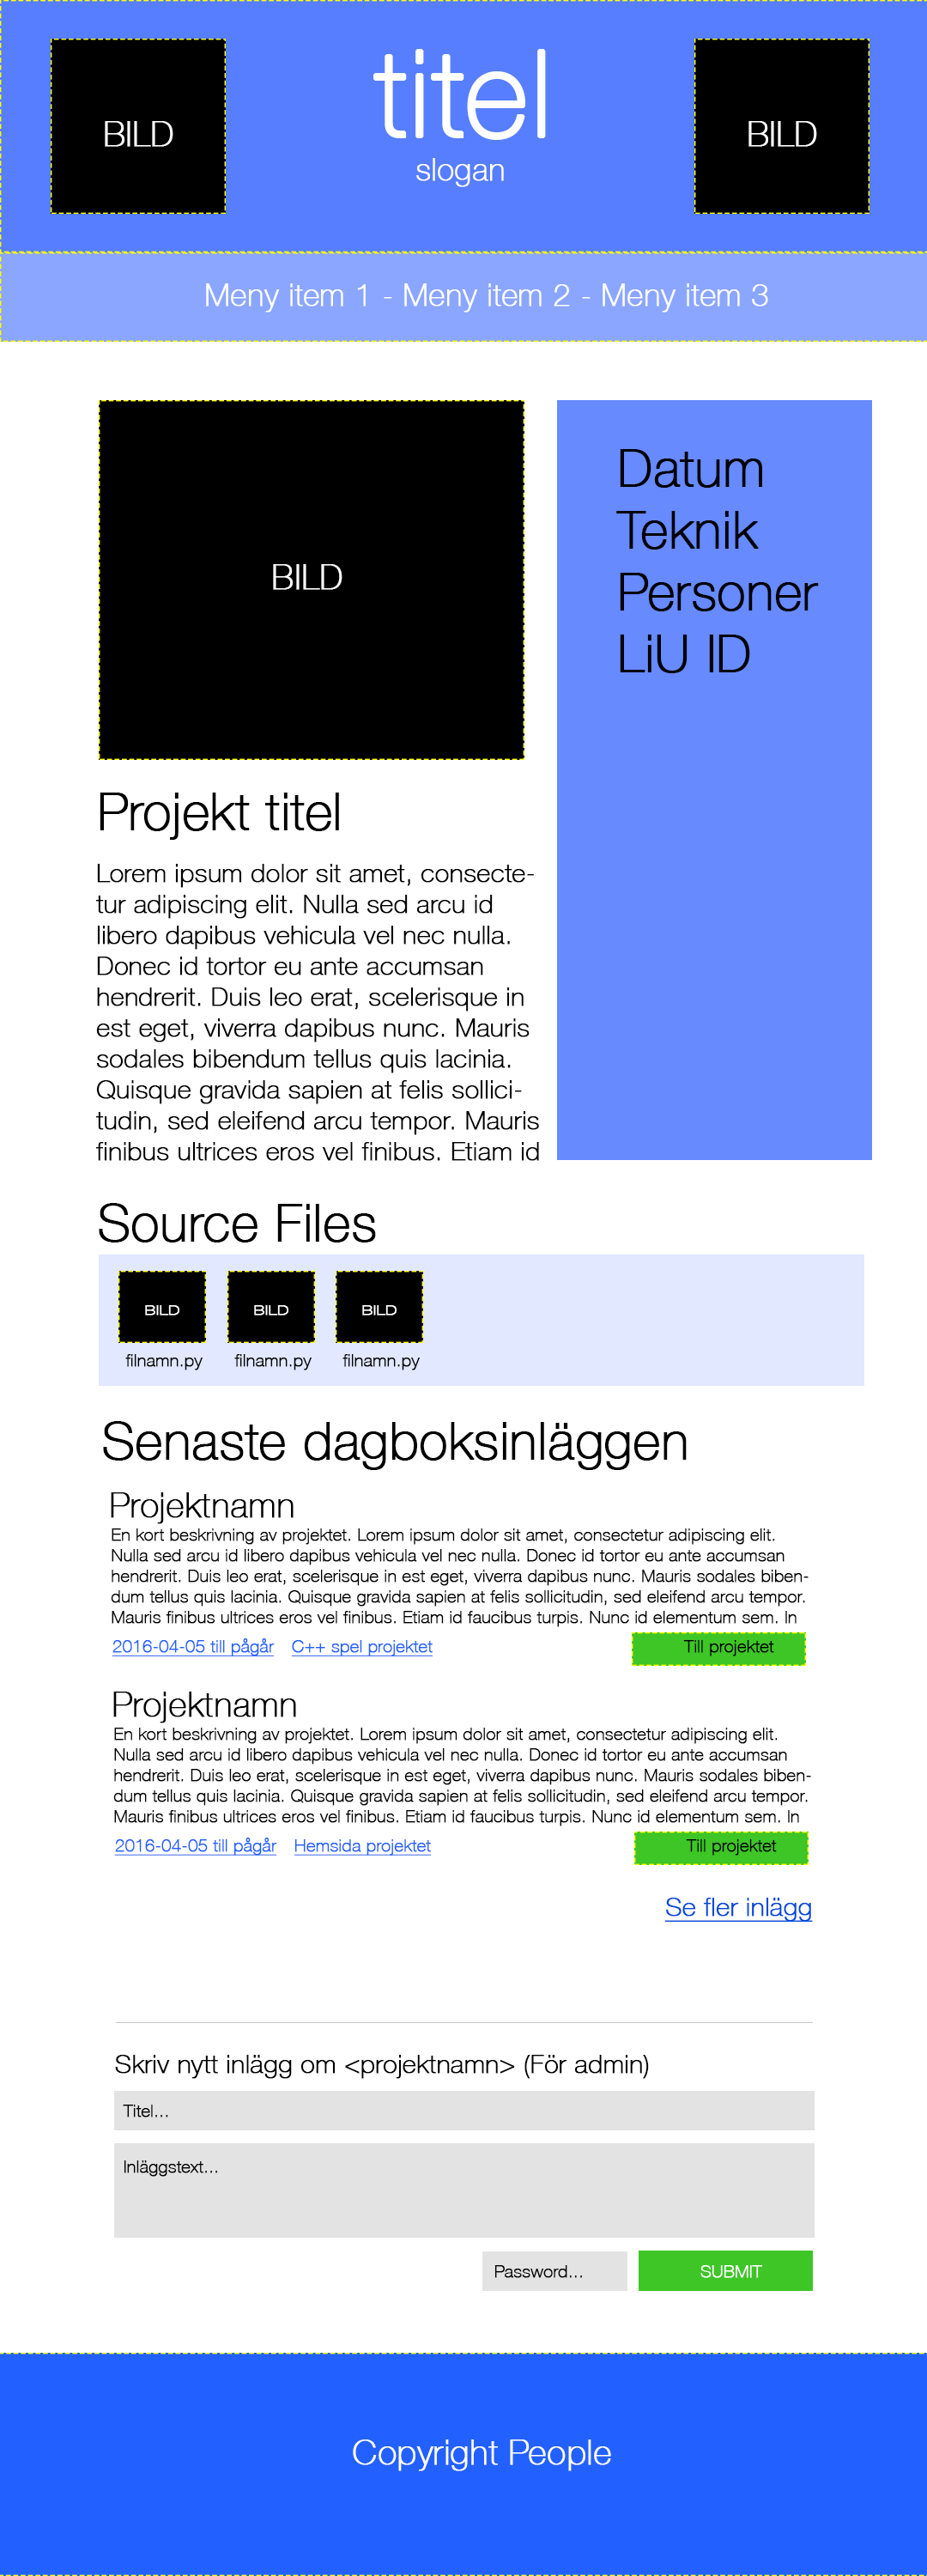
\includegraphics[height=14cm]{projekt-id.png}

\end{document}
